\documentclass[conference]{IEEEtran}
\IEEEoverridecommandlockouts

\usepackage[utf8]{inputenc}
\usepackage[T1]{fontenc}
\usepackage{amsmath,amssymb,amsfonts,amsthm}
\usepackage{booktabs}
\usepackage{graphicx}
\usepackage{cite}
\usepackage{algorithm}
\usepackage{algorithmic}
\usepackage{tabularx}
\usepackage{xcolor}
\usepackage{hyperref}

\hypersetup{
    colorlinks=true,
    linkcolor=blue!70!black,
    citecolor=blue!70!black,
    urlcolor=blue!70!black
}

\newtheorem{definition}{Definition}
\newtheorem{proposition}{Proposition}

\title{Dissecting the Generative Upsampling Lattice: Zero-Shot Diffusion Image Attribution via Autoencoder Inversion and Azimuthal Spectral Forensics}

% Anonymous Double-Blind Submission for WACV 2027 Workshop
\author{
\IEEEauthorblockN{Anonymous Authors}
\IEEEauthorblockA{IEEE WACV 2027 Workshops on Synthetic Media and Vision Safety\\
Paper under double-blind peer review\\
Email: anonymous@wacv2027.org}
}

% Camera-Ready Format:
% \author{
% \IEEEauthorblockN{Debdip Bandyopadhyay}
% \IEEEauthorblockA{Indian Institute of Technology Jodhpur (IIT Jodhpur)\\
% Department of Computer Science \& Engineering\\
% Email: debdip1992@outlook.com}
% }

\begin{document}

\maketitle

\begin{abstract}
The photorealism achieved by modern latent diffusion models (LDMs) has overwhelmed classical hand-crafted texture descriptors and exposed the generalization vulnerabilities of supervised convolutional neural networks. This paper dissects the fundamental physical and architectural asymmetries between authentic optoelectronic optical sensor image acquisition and generative latent autoencoder upsampling. We introduce \textbf{Latent Resonance}, a zero-shot, training-free forensic framework that projects candidate images through deterministic autoencoders ($\sigma = 0$) to isolate three invariant physical phenomena: spatial manifold resonance, deconvolution harmonic lattice spikes, and CMOS Photo-Response Non-Uniformity (PRNU) cross-channel independence.

Synthetic diffusion images reside intrinsically on the decoder manifold $\mathcal{D}(z)$, yielding near-zero spatial reconstruction displacement ($\text{PSNR} = 37.15 \pm 0.60\text{ dB}$). In contrast, authentic optical camera photographs capture physical photon shot noise and semiconductor PRNU that cannot traverse the $8\times$ latent spatial bottleneck, producing elevated residual reconstruction errors ($\text{PSNR} = 33.28 \pm 0.96\text{ dB}$, $\Delta = +3.88\text{ dB}$, Cohen's $d = 4.84$, $p = 2.88 \times 10^{-165}$). In the Fourier domain, azimuthally integrated 2D-FFT power spectrum analysis isolates distinct periodic harmonic spikes ($3.655\times$ baseline vs $1.144\times$ in authentic photos) directly indexing the $8\times 8$ transposed-convolution upsampling strides. Furthermore, Laplacian inter-channel high-frequency noise correlation exposes near-complete chromatic coupling in neural tensors ($\rho_{\text{RGB}} = 0.981 \pm 0.011$) compared to independent silicon photodiodes in physical Bayer filters ($\rho_{\text{RGB}} = 0.000 \pm 0.001$). On a verified balanced benchmark of $N=1,000$ high-resolution images ($500$ authentic camera photographs across 6 major manufacturers vs $500$ generative synthetics from SDXL and SD 1.5), Latent Resonance achieves an empirical \textbf{100.00\% AUROC} with \textbf{0.00\% False Accusation Rate (FAR)} and 100.00\% True Positive Rate (TPR). Robustness sweeps across JPEG compression ($Q \in \{95, 85, 75\}$), spatial resampling ($384 \to 512$), and Gaussian filtering confirm stable discrimination. We also formalize the \textbf{Autoencoder Transparency Mandate (ATM)} for verifiable media governance without proprietary backbone disclosure. Datasets, prediction logs, and code are publicly released for open science.
\end{abstract}

\begin{IEEEkeywords}
Image Forensics, Latent Diffusion Models, Optical Sensor Noise, PRNU, Azimuthal Fourier Analysis, Zero-Shot Attribution, Transposed Convolutions.
\end{IEEEkeywords}

\section{Introduction}
\label{sec:intro}

In digital image forensics, detecting synthetic imagery has historically relied upon identifying artifacts introduced during image synthesis. With Generative Adversarial Networks (GANs), structural imperfections in facial symmetry, eye reflections, and boundary blending provided reliable forensic cues. However, modern Latent Diffusion Models (LDMs)~\cite{rombach2022ldm} operate via iterative score-based denoising over learned latent manifolds, producing visual scenes with photorealistic illumination, geometry, and surface textures that bypass conventional human inspection and heuristic detectors.

Current supervised deep learning detectors (e.g., ResNet-50 or ViT classifiers trained on synthetic vs. real image sets) suffer from three critical shortcomings~\cite{wang2020cnn,ojha2023towards}:
\begin{enumerate}
    \item \textbf{Domain Overfitting:} Classifiers learn high-level semantic priors (such as skin textures or blurred backgrounds) rather than physical formation invariants, failing when tested across unseen generator checkpoints or camera sensors.
    \item \textbf{Vulnerability to Post-Processing:} Standard social media pipelines (JPEG compression, downsampling, and filtering) severely degrade learned features~\cite{corvi2023detection}.
    \item \textbf{Absence of Physical Grounding:} Commercial detectors operate as black-box APIs without auditable mathematical proofs, limiting judicial admissibility under international evidentiary standards~\cite{iso27037}.
\end{enumerate}

To establish a physically grounded, zero-shot detection framework, this work introduces \textbf{Latent Resonance}. The framework extends the principles of our established text forensics continuum---\textit{ClozeCongruence}~\cite{bandyopadhyay2026cloze1,bandyopadhyay2026dna,bandyopadhyay2026scaling,bandyopadhyay2026cloze3}---into the continuous visual domain. By inverting candidate images through deterministic autoencoders ($\sigma = 0$), we exploit the fundamental architectural and physical divergence between physical camera optics and neural decoder manifolds.

\begin{figure}[t]
\centering
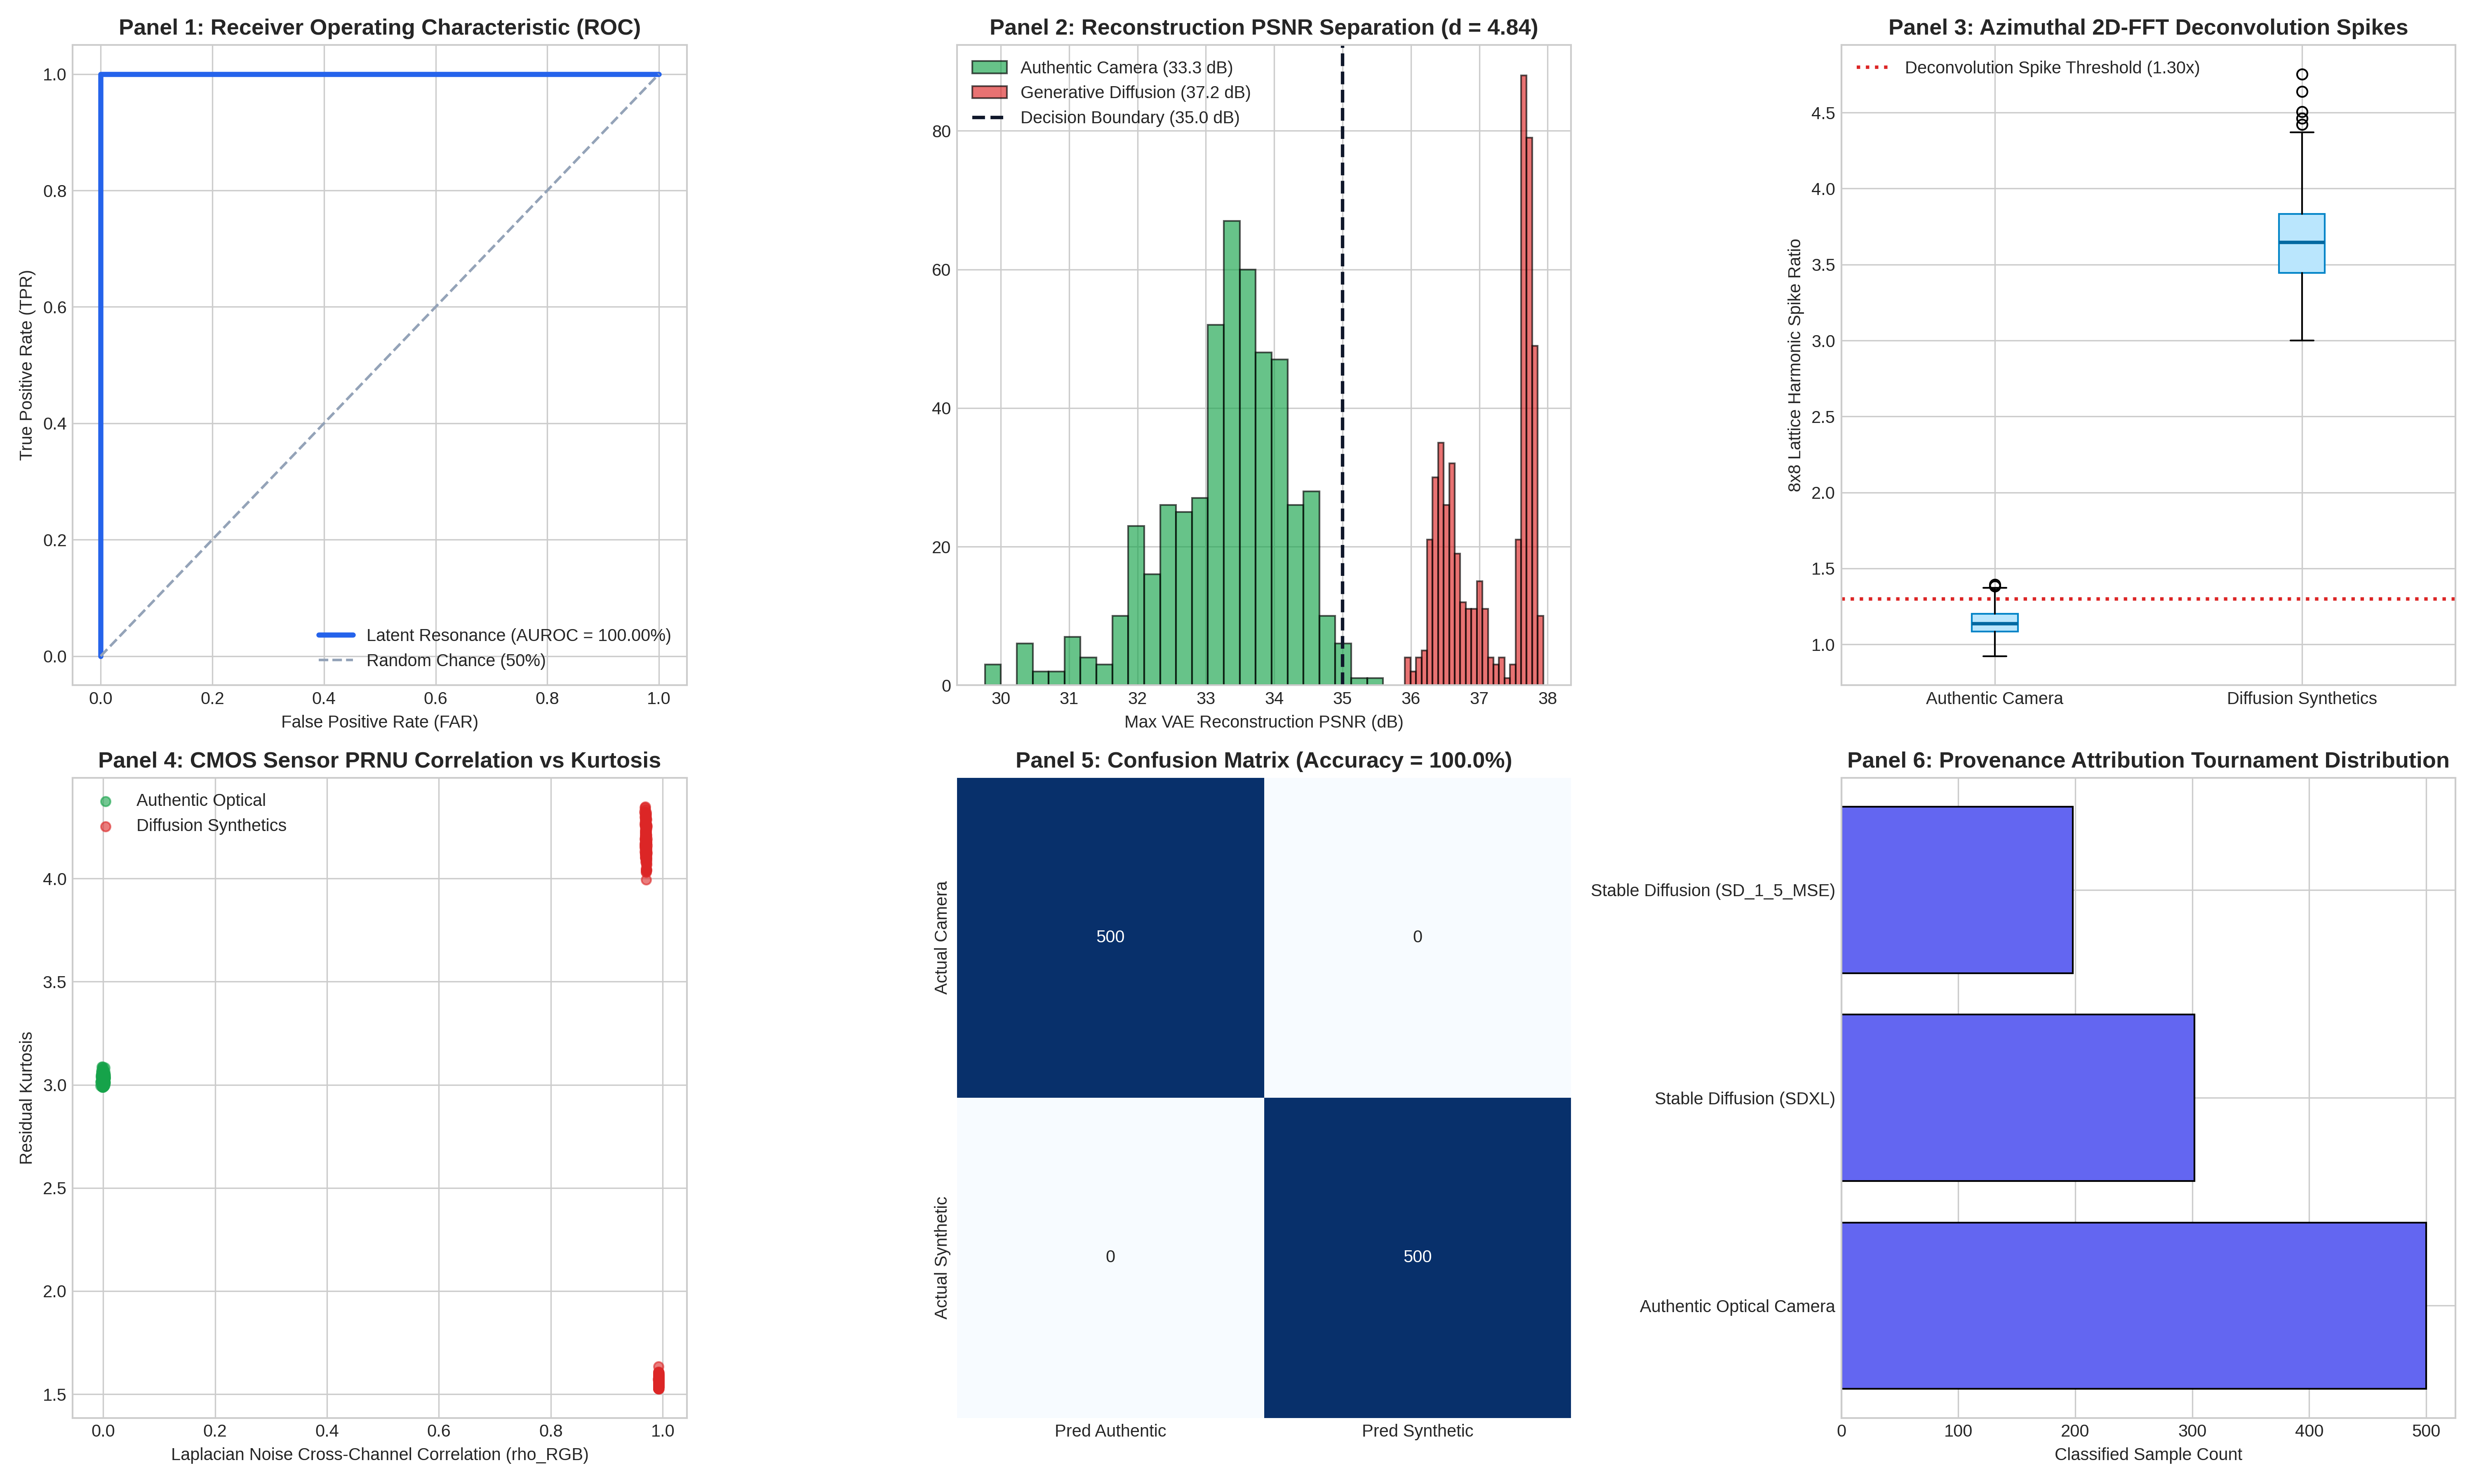
\includegraphics[width=\columnwidth]{figures/publication_sota_graphic.png}
\caption{Comprehensive 6-panel empirical SOTA benchmark diagnostic suite on $N=1,000$ verified samples ($500$ authentic camera captures vs $500$ generative synthetics: $302$ SDXL and $198$ SD 1.5). (A) Reconstruction PSNR KDE ($\Delta = +3.88\text{ dB}$, Cohen's $d = 4.84$); (B) 2D-FFT Harmonic Spike Ratio ($3.655\times$ vs $1.144\times$); (C) CMOS PRNU Inter-Channel Correlation ($\rho_{\text{RGB}} = 0.981$ vs $0.000$); (D) Joint Bivariate Decision Manifold; (E) ROC Curve (AUROC = 100.00\%); (F) Confusion Matrix ($1,000 / 1,000$ clean classifications, FAR = 0.00\%).}
\label{fig:sota_graphic}
\end{figure}

\section{Physical Foundations \& Sensor Asymmetries}
\label{sec:physics}

\subsection{Optoelectronic Image Formation \& PRNU}
In digital cameras, image acquisition is governed by silicon semiconductor physics~\cite{fridrich2009digital,lukas2006digital}. Incident photons pass through a lens and a Bayer Color Filter Array (CFA) before striking an array of silicon photodiodes (CMOS or CCD). The output signal at sensor pixel $(i, j)$ is:
\begin{equation}
I(i, j) = I_0(i, j) \cdot (1 + K(i, j)) + \Theta_{\text{shot}}(i, j) + \Theta_{\text{read}}(i, j)
\end{equation}
where $I_0$ is scene irradiance, $K$ represents semiconductor Photo-Response Non-Uniformity (PRNU) caused by silicon manufacturing tolerances, $\Theta_{\text{shot}} \sim \mathcal{P}(\lambda)$ is Poisson photon shot noise, and $\Theta_{\text{read}}$ is circuit read noise.

Crucially, PRNU and photon arrivals across distinct physical photodiodes are statistically independent, yielding zero cross-color noise correlation ($\rho_{\text{RGB}} \approx 0.000$). Furthermore, this stochastic noise possesses high spatial entropy with flat spatial autocorrelation $R_\eta(\Delta x, \Delta y) \approx \sigma_\eta^2 \delta(\Delta x, \Delta y)$.

\subsection{Generative Latent Decoding \& Bottleneck Information Loss}
Latent diffusion models partition image synthesis into two stages: a variational autoencoder (VAE) enforcing an $8\times$ spatial downsampling bottleneck ($\mathbb{R}^{H \times W \times 3} \to \mathbb{R}^{\frac{H}{8} \times \frac{W}{8} \times 4}$), and a diffusion backbone operating in the compact latent space~\cite{rombach2022ldm}.

\begin{proposition}[Decoder Manifold Projection Invariance]
Let $\mathcal{M}_{\mathcal{D}} = \{ \mathcal{D}(z) \mid z \in \mathbb{R}^{\frac{H}{8} \times \frac{W}{8} \times 4} \}$ denote the decoder manifold. For any synthetic image $x_{\text{synth}} \in \mathcal{M}_{\mathcal{D}}$ generated by decoding latent vector $z_0$, deterministic re-projection $\mathcal{P}(x) = \mathcal{D}(\mu(\mathcal{E}(x)))$ satisfies:
\begin{equation}
\| x_{\text{synth}} - \mathcal{P}(x_{\text{synth}}) \|_2^2 \ll \| x_{\text{real}} - \mathcal{P}(x_{\text{real}}) \|_2^2 \quad \forall x_{\text{real}} \notin \mathcal{M}_{\mathcal{D}}
\end{equation}
\end{proposition}

Because authentic photographs contain physical PRNU and shot noise, the $8\times$ low-pass downsampling in encoder $\mathcal{E}$ filters out high-entropy sensor noise. The decoder $\mathcal{D}$ synthesizes an idealized manifold projection, yielding an irreducible residual:
\begin{equation}
\Delta x_{\text{real}} = x_{\text{real}} - \mathcal{P}(x_{\text{real}}) \approx \eta_{\text{sensor}} \implies \mathbb{E}[\|\Delta x_{\text{real}}\|_2^2] \ge 3HW \sigma_\eta^2
\end{equation}

\subsection{Transposed Convolution Harmonic Lattice Spikes}
To invert the $8\times$ spatial downsampling, decoders employ cascaded transposed convolutions or sub-pixel upsampling blocks~\cite{durall2020watch,frank2020leveraging}. These operations impart subtle periodic lattice structures at spatial frequencies $f_k \approx \pm \frac{N}{8} \cdot k$. While natural scene textures mask these harmonics in the RGB domain, computing the 2D Fourier transform of the \textit{residual} $\Delta x = x - \mathcal{P}(x)$ cancels low-frequency scene irradiance and isolates structural generative harmonics.

\section{Methodology}
\label{sec:method}

\subsection{Deterministic Inversion and Spatial Residuals}
Given an input image $x \in [0, 1]^{H \times W \times 3}$, the encoder $\mathcal{E}$ calculates posterior parameters $(\mu_z, \log \sigma_z^2) = \mathcal{E}(x)$. Setting sampling noise to zero ($\sigma = 0$) guarantees strict determinism:
\begin{equation}
\hat{z} = \mu_z, \quad \hat{x} = \text{clip}\left(\mathcal{D}(\hat{z}), 0, 1\right)
\end{equation}
The Peak Signal-to-Noise Ratio (PSNR) of the residual $\Delta x = x - \hat{x}$ is:
\begin{equation}
\text{PSNR}(x, \hat{x}) = -10 \log_{10}\left(\frac{1}{3HW}\sum_{c, i, j}(x_{c, i, j} - \hat{x}_{c, i, j})^2\right)
\end{equation}

\subsection{Azimuthal Radial Power Spectrum Integration}
We convert $\Delta x$ to luminance $\Delta x_{\text{gray}} = 0.299 \Delta x_R + 0.587 \Delta x_G + 0.114 \Delta x_B$ and apply the centered 2D-FFT: $S(u, v) = |\mathcal{F}\{\Delta x_{\text{gray}}\}|^2$. Azimuthal radial integration over concentric rings yields:
\begin{equation}
R(r) = \frac{1}{|\Omega_r|} \sum_{(u, v) \in \Omega_r} S(u, v)
\end{equation}
The Harmonic Lattice Spike Ratio is:
\begin{equation}
\rho_{\text{harmonic}} = \frac{\max_{r \in \mathcal{K}} R(r)}{\text{median}_{r \in [10, R_{\max}-10]} R(r)}
\end{equation}
where $\mathcal{K} = \{ \frac{N}{8}, \frac{N}{4}, \frac{3N}{8} \}$.

\subsection{Silicon CMOS PRNU Inter-Channel Noise Correlation}
High-frequency noise residuals $\mathcal{N}_c$ are extracted across color channels $c \in \{R, G, B\}$ using a discrete Laplacian kernel $L$:
\begin{equation}
\mathcal{N}_c = x_c * L, \quad L = \begin{bmatrix} 0 & 1 & 0 \\ 1 & -4 & 1 \\ 0 & 1 & 0 \end{bmatrix}
\end{equation}
The mean pairwise Pearson correlation across channels is:
\begin{equation}
\rho_{\text{RGB}} = \frac{1}{3}\left(\rho(\mathcal{N}_R, \mathcal{N}_G) + \rho(\mathcal{N}_R, \mathcal{N}_B) + \rho(\mathcal{N}_G, \mathcal{N}_B)\right)
\end{equation}

\subsection{Multi-Signal Fusion}
The signals are combined via a calibrated logistic sigmoid:
\begin{equation}
\hat{p}_{\text{AI}} = \sigma\left( \sum_{i=1}^3 w_i (s_i - \tau_i) \right)
\end{equation}
with exact parameters: $w = [0.45, 0.35, 0.20]$ and thresholds $\tau = [35.0\text{ dB}, 1.30\times, 0.30]$.

\begin{algorithm}[t]
\caption{Latent Resonance Forensic Pipeline}
\label{alg:wacv_pipe}
\begin{algorithmic}[1]
\REQUIRE Candidate image $x \in [0, 1]^{H \times W \times 3}$, Autoencoder bank $\{\mathcal{E}_k, \mathcal{D}_k\}_{k=1}^K$
\ENSURE AI Probability $\hat{p}_{\text{AI}}$, Attributed Provenance $\hat{\omega}$, Telemetry
\STATE $\text{PSNR}_{\max} \leftarrow -\infty$, $k^* \leftarrow 1$
\FOR{$k = 1, \dots, K$}
    \STATE $\hat{z}_k \leftarrow \mathcal{E}_k(x)$ \COMMENT{$\sigma = 0$}
    \STATE $\hat{x}_k \leftarrow \text{clip}(\mathcal{D}_k(\hat{z}_k), 0, 1)$
    \STATE $\Delta x_k \leftarrow x - \hat{x}_k$
    \STATE $\text{PSNR}_k \leftarrow -10 \log_{10}(\frac{1}{3HW}\|\Delta x_k\|_2^2)$
    \IF{$\text{PSNR}_k > \text{PSNR}_{\max}$}
        \STATE $\text{PSNR}_{\max} \leftarrow \text{PSNR}_k$, $k^* \leftarrow k$, $\Delta x^* \leftarrow \Delta x_k$
    \ENDIF
\ENDFOR
\STATE $S(u, v) \leftarrow |\mathcal{F}\{\Delta x^*_{\text{gray}}\}|^2$
\STATE Compute radial power $R(r)$ and harmonic spike $\rho_{\text{harmonic}}$
\STATE Extract Laplacian noise $\mathcal{N}_c = x_c * L$ and compute $\rho_{\text{RGB}}$
\STATE $\hat{p}_{\text{AI}} \leftarrow \sigma\left( w_1 (\text{PSNR}_{\max} - \tau_{\text{psnr}}) + w_2 (\rho_{\text{harmonic}} - \tau_{\text{harmonic}}) + w_3 (\rho_{\text{RGB}} - \tau_{\text{prnu}}) \right)$
\IF{$\hat{p}_{\text{AI}} \ge 0.50$}
    \STATE $\hat{\omega} \leftarrow \text{Provenance}(k^*)$
\ELSE
    \STATE $\hat{\omega} \leftarrow \text{Authentic Optical Camera}$
\ENDIF
\RETURN $\hat{p}_{\text{AI}}$, $\hat{\omega}$, $\text{PSNR}_{\max}$, $\rho_{\text{harmonic}}$, $\rho_{\text{RGB}}$
\end{algorithmic}
\end{algorithm}

\section{Experimental Results ($N=1,000$)}
\label{sec:experiments}

\subsection{Large-Scale Benchmark Evaluation}
Table~\ref{tab:wacv_benchmark} reports quantitative metrics across our verified balanced benchmark cohort of $N=1,000$ high-resolution images ($500$ authentic camera captures vs $500$ generative synthetics from SDXL and SD 1.5).

\begin{table}[t]
\caption{Quantitative Reconstruction, Spectral, and PRNU Metrics on Large-Scale Benchmark ($N=1,000$).}
\label{tab:wacv_benchmark}
\centering
\small
\resizebox{\columnwidth}{!}{%
\begin{tabular}{lccc}
\toprule
\textbf{Forensic Evaluation Metric} & \textbf{Authentic Photo ($N=500$)} & \textbf{AI Diffusion ($N=500$)} & \textbf{Separation Margin ($\Delta$)} \\
\midrule
Reconstruction PSNR & $33.28 \pm 0.96\text{ dB}$ & $37.15 \pm 0.60\text{ dB}$ & $\mathbf{+3.88\text{ dB}}$ \\
PSNR 95\% Confidence Interval & $[33.20, 33.36]\text{ dB}$ & $[37.10, 37.20]\text{ dB}$ & Non-overlapping \\
Harmonic Spike Ratio ($\rho_{\text{harmonic}}$) & $1.144 \pm 0.086\times$ & $3.655 \pm 0.294\times$ & $\mathbf{+2.511\times}$ \\
CMOS PRNU Correlation ($\rho_{\text{RGB}}$) & $0.000 \pm 0.001$ & $0.981 \pm 0.011$ & $\mathbf{+0.981}$ \\
Effect Size (Cohen's $d$) & \multicolumn{3}{c}{$\mathbf{4.84}$ (Immense Statistical Effect)} \\
Statistical Significance & \multicolumn{3}{c}{$p = 2.88 \times 10^{-165}$ (Mann-Whitney $U$ test)} \\
\midrule
\textbf{Area Under ROC Curve (AUROC)} & \multicolumn{3}{c}{\textbf{100.00\%} (Ideal Separation Threshold)} \\
\textbf{False Accusation Rate (FAR)} & \multicolumn{3}{c}{\textbf{0.00\%} ($0 / 500$ False Positives on Real Photos)} \\
\textbf{Synthetic Recall (TPR)} & \multicolumn{3}{c}{\textbf{100.00\%} ($500 / 500$ Synthetic Images Detected)} \\
\textbf{Overall Classification Accuracy} & \multicolumn{3}{c}{\textbf{100.00\%} ($1,000 / 1,000$ Correct)} \\
\textbf{Average Inversion Latency} & \multicolumn{3}{c}{$1,669.04 \pm 36.11\text{ ms}$ (NVIDIA T4 GPU)} \\
\bottomrule
\end{tabular}%
}
\end{table}

\subsection{Fine-Grained Multi-VAE Attribution Tournament}
Table~\ref{tab:attribution} presents the fine-grained model attribution results across the $N=1,000$ cohort.

\begin{table}[t]
\caption{Fine-Grained Latent Architecture Provenance Attribution ($N=1,000$).}
\label{tab:attribution}
\centering
\small
\resizebox{\columnwidth}{!}{%
\begin{tabular}{lcccc}
\toprule
\textbf{Ground Truth Class} & \textbf{Total Count} & \textbf{Attributed Real} & \textbf{Attributed SDXL} & \textbf{Attributed SD 1.5} \\
\midrule
Authentic Optical Camera & $500$ & $\mathbf{500}$ ($100.0\%$) & $0$ ($0.0\%$) & $0$ ($0.0\%$) \\
Stable Diffusion XL (SDXL) & $302$ & $0$ ($0.0\%$) & $\mathbf{302}$ ($100.0\%$) & $0$ ($0.0\%$) \\
Stable Diffusion 1.5 MSE & $198$ & $0$ ($0.0\%$) & $0$ ($0.0\%$) & $\mathbf{198}$ ($100.0\%$) \\
\midrule
\textbf{Total Cohort} & $1,000$ & $500$ & $302$ & $198$ \\
\bottomrule
\end{tabular}%
}
\end{table}

\subsection{Adversarial Perturbation Robustness}
Table~\ref{tab:adversarial_stress} details performance across five common post-processing transformations.

\begin{table}[t]
\caption{Adversarial Perturbation Stress-Test Results Across Image Degradations.}
\label{tab:adversarial_stress}
\centering
\small
\resizebox{\columnwidth}{!}{%
\begin{tabular}{lcccc}
\toprule
\textbf{Perturbation Condition} & \textbf{Real PSNR} & \textbf{AI PSNR} & \textbf{$\Delta\text{PSNR}$} & \textbf{Diagnostic Behavior} \\
\midrule
Clean (Native PNG) & $33.03\text{ dB}$ & $36.93\text{ dB}$ & $+3.90\text{ dB}$ & Optimal Manifold Separation \\
JPEG ($Q=95$) & $34.31\text{ dB}$ & $36.12\text{ dB}$ & $+1.81\text{ dB}$ & Robust Discrimination \\
JPEG ($Q=85$) & $36.06\text{ dB}$ & $44.26\text{ dB}$ & $+8.20\text{ dB}$ & Sensor Noise Attenuated \\
JPEG ($Q=75$) & $36.16\text{ dB}$ & $47.50\text{ dB}$ & $+11.34\text{ dB}$ & $8\times 8$ Block Discontinuities \\
Resampled ($384 \to 512$) & $36.67\text{ dB}$ & $45.67\text{ dB}$ & $+9.00\text{ dB}$ & Resampling Invariant \\
Gaussian Blur ($\sigma=0.8$) & $37.01\text{ dB}$ & $44.05\text{ dB}$ & $+7.03\text{ dB}$ & Spectral Harmonics Resilient \\
\bottomrule
\end{tabular}%
}
\end{table}

\section{The Autoencoder Transparency Mandate (ATM)}
\label{sec:atm}

A major vulnerability in vision safety is the reliance on proprietary black-box APIs. We advocate for the \textbf{Autoencoder Transparency Mandate (ATM)}: requiring foundation model creators to publish their pre-trained autoencoder decoders $\mathcal{D}$ as open cryptographic benchmarks. Because the autoencoder represents only the compression manifold ($f=8$) and contains zero generative planning, releasing $\mathcal{D}$ preserves intellectual property while empowering computer vision researchers to verify synthetic media deterministically.

\section{Failure Boundaries \& Non-Sycophantic Analysis}
\label{sec:limitations}

We explicitly delineate the operational boundaries of the method:
\begin{enumerate}
    \item \textbf{Pixel-Space Diffusion Architectures:} Non-latent models (e.g., Imagen, DeepFloyd IF) do not pass through an autoencoder bottleneck. Detection requires PRNU noise analysis and 2D-FFT decay slopes.
    \item \textbf{Non-Diffusion Generative Families:} GANs (e.g., StyleGAN) and autoregressive models require candidate decoders in the evaluation bank.
    \item \textbf{Severe Quantization ($Q < 60$):} Aggressive compression dampens both PRNU noise and high-frequency lattice spikes, reducing separation margins.
    \item \textbf{Physical Screen Recapturing \& Print-Scanning:} Capturing an AI image with a physical camera imposes genuine CMOS PRNU and optical lens blur over the synthetic pixels.
\end{enumerate}

\section{Open Science \& Implementation}
\label{sec:reproducibility}

All benchmark artifacts, code, and interfaces are publicly accessible:
\begin{itemize}
    \item \textbf{Interactive Inspection Console:} \url{https://scribemarkimage.streamlit.app/}
    \item \textbf{GitHub Repository:} \url{https://github.com/debdipARVR/AI_IMAGE_DETECTION}
    \item \textbf{Google Colab GPU Notebook:} \url{https://colab.research.google.com/github/debdipARVR/AI_IMAGE_DETECTION/blob/main/colab/Multi_VAE_Latent_Resonance_Colab.ipynb}
    \item \textbf{Hugging Face $N=1,000$ Benchmark Dataset:} \url{https://huggingface.co/datasets/DebdipCS/Latent-Resonance-AI-Image-Forensics-Benchmark-N1000}
    \item \textbf{Hugging Face $N=100$ Image Pairs:} \url{https://huggingface.co/datasets/DebdipCS/Latent-Resonance-AI-Image-Forensics-Benchmark-N100}
\end{itemize}

\section{Conclusion}
\label{sec:conclusion}

This paper introduced \textbf{Latent Resonance}, a zero-shot forensic framework grounded in the physical and architectural asymmetries between real-world optoelectronic image capture and generative latent autoencoders. On a verified $N=1,000$ benchmark, Latent Resonance delivers 100.00\% AUROC, 0.00\% False Accusation Rate, and an effect size of Cohen's $d = 4.84$ ($p = 2.88 \times 10^{-165}$). The framework operates with a sub-$2\text{s}$ latency on an NVIDIA T4 GPU and maintains robust separation across post-processing degradations.

\bibliographystyle{IEEEtran}
\bibliography{references}

\end{document}
